\begin{figure}
    \centering
        \vspace{-3mm}
    \begin{subfigure}{.45\textwidth}
        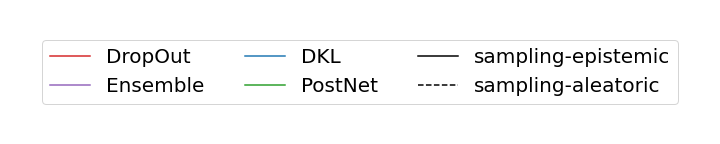
\includegraphics[width=\textwidth]{sections/011_icml2022/resources/sampling-legend.png}
    \end{subfigure}
    \vspace{-3mm}
    
    \begin{subfigure}{.245\textwidth}
        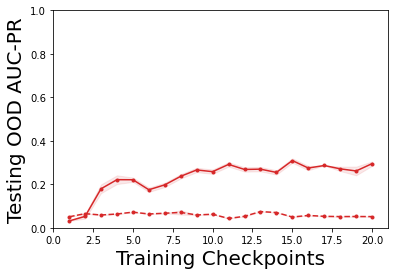
\includegraphics[width=\textwidth]{sections/011_icml2022/resources/DropOut-CartPoleOOD-v0-AUC-PR-out-epistemic_-testing-strategy.png}
    \end{subfigure}
    \begin{subfigure}{.245\textwidth}
        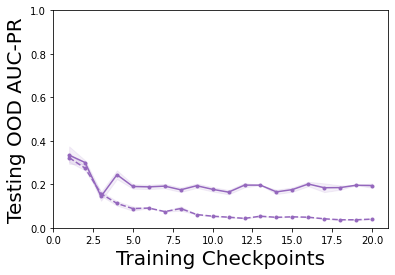
\includegraphics[width=\textwidth]{sections/011_icml2022/resources/Ensemble-CartPoleOOD-v0-AUC-PR-out-epistemic_-testing-strategy.png}
    \end{subfigure}
    \begin{subfigure}{.245\textwidth}
        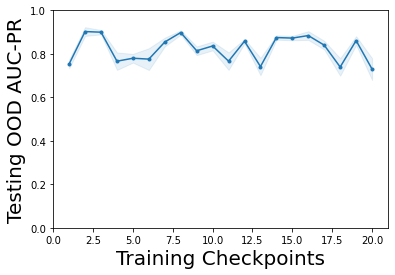
\includegraphics[width=\textwidth]{sections/011_icml2022/resources/DKL-CartPoleOOD-v0-AUC-PR-out-epistemic_-testing-strategy.png}
    \end{subfigure}
    \begin{subfigure}{.245\textwidth}
        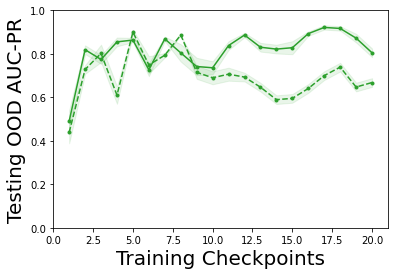
\includegraphics[width=\textwidth]{sections/011_icml2022/resources/PostNet-CartPoleOOD-v0-AUC-PR-out-epistemic_-testing-strategy.png}
    \end{subfigure}
        \vspace{-3mm}
    \caption{Comparison of the OOD performance on CartPole. The four uncertainty methods use the sampling-aleatoric or sampling-epistemic strategies at both training and testing time. Ideally, an uncertainty aware-model should achieve high testing reward and high OOD AUC-PR detection score.}
    \label{fig:strategy-testing-ood-auc-pr-performance-cartpole}
        \vspace{-3mm}
\end{figure}